\section{Uvod}

Prilikom razvoja operativnih sistema, drajvera, bootloader-a i drugih kritičnih sistemskih softvera, koriste se jezici niskog nivoa kao što su C i C++.
Tokom godina Microsoft je uvideo da je preko 70\% bezbednosnih slabosti nastalo neadekvatnim rukovanjem memorijom [1]. Najčešći primeri su korišćenje memorije 
nakon oslobadjanja, višestruko oslobadjanje iste memorijske lokacije, nebezbedna aritemetika pokazivačima, curenje memorije i prepopunjavanje bafera.
Takođe sa stanovišta paralelnog programiranja, oba jezika zahtevaju pedantno rukovanje muteksima i semaforima jer u suprotnom nastaju novi problemi poput 
problema trke i problema medjusobnog čekanja. Problem trke nastaje kada dve ili više niti pokušavaju da izmene podatak istovremeno, pri čemu redosled izvršavanja 
utiče na ishod. Problem medjusobnog čekanja nastaje kada dve ili više niti čekaju jednu na drugu da oslobode resurse pri čemu se izvršavanje 
zaustavlja.

Programski jezik C nema ugrađene odbrambene mehanizme od prethodno navedenih problema. Pridržavanje C standardu otvara mogućnost za uporedo 
korišćenje GCC i Clang kompajlera čime se dobija uvid u relativno štura upozorenja od strane oba programska prevodioca.
Sa druge strane programski jezik C++ uprkos dodavanju primitiva kao što su \verb|unique_ptr|, \verb|shared_ptr| i \verb|weak_ptr|, i dalje zbog interoperabilnosti 
sa starijim standardima ili bibliotekama zahteva korišćenje sirovih pokazivača. Vremenom su se razvili softverski obrasci kao što je \verb|Scope-bound Resource Management|
koje nastoji da dobrim praksama umanji šansu da se problem prvobitno desi. Naime, korisnik jezika nije primoran da softverski obrazac upotrebi ili čak zna 
za njegovo postojanje.

Rust je programski jezik stvoren s jasnim ciljem: da reši probleme povezane sa memorijskom i paralelnom bezbednošću. 
Njegova podrazumevana upotreba garantuje bezbednost zahvaljujući robustom sistemu tipova, inovativnom načinu upravljanja memorijom i striktnog \verb|rustc| kompajlera.
Za razliku od C i C++ koji često daju nejasne poruke o greškama, Rust nudi izuzetno precizne dijagnostičke poruke koje tačno ukazuju na mesto 
greške i nude potencijalna rešenja.

Sa obzirom na značajne inovacije koje donosi Rust jezik, detaljno razumevanje njegovog internog funkcionisanja je od velikog značaja. Rust-ove garancije 
bezbednosti nisu magične, primarno proizilaze iz sistema pravila \verb|borrow-checker|-a, životnih vekova i osobina koje garantuju bezbednost nekog tipa 
u paralelnom okruženju. Rust nudi mnoge napredne funkcije kao što su makroi, unsafe kod, FFI (Foreign Function Interface) za interakciju sa C kodom. Detaljno razumevanje osnova jezika i njegovog internog funkcionisanja je preduslov za efikasno korišćenje ovih naprednih 
mogućnosti na siguran i efikasan način. Na primer, kada se koristi unsafe blok, programer preuzima odgovornost za bezbednost memorije, 
što zahteva duboko razumevanje načina na koji Rust obično to radi.

Zanimljivo je da je prva verzija Rust kompajlera bila napisana u O'Caml-u, ali su sve naredne verzije razvijene u samom Rust-u. 
Važno je napomenuti da je Rust zapravo samo frontend za LLVM. LLVM predstavlja skup modularnih i višekratno upotrebljivih tehnologija za izgradnju kompajlera. 
Rust se u potpunosti oslanja na LLVM za generisanje mašinskog koda, dok je kompletan frontend Rust-a napisan od nule.

Medjureprezentacije izvornog koda u Rust-u obuhvataju različite prikaze korisničkog koda koji omogu\hyp{}ćavaju ključne funkcionalnosti jezika, 
uključujući proveru tipova, dijagnostiku grešaka, automatsku dealo\hyp{}kaciju memorije i druge ergonomske i funkcionalne karakteristike.

\newpage

\section{Pozadina}

U ovoj sekciji obradjuje se pozadina iza \verb|Rust| jezika, zvaničnog menadžera paketa \verb|Cargo| i 
LLVM seta alata.

\subsection{Rust jezik}

\verb|Rust| je statički tipiziran jezik koji je nastao 2006. godine kao lični projekat \verb|Graydon| \verb|Hoare|-a, radnika kompanije 
Mozilla. Uvidevši potencijal jezika, Mozila je započela sponzorisanje projekta 2010. godine kada je jezik i javno 
predstavljen \cite{rust-language}. \verb|Rust| je jezik niskog nivoa koji se fokusira na memorijsku bezbednost
i bezbedan paralelizam bez oslanjanja na skupljač smeća (\verb|garbage| \verb|collector|). Skupljač smeća 
obično uvodi lakoću programiranja na uštrb nedeterminističkih performansi usled oslobadjanja memorije 
sa \verb|heap|-a, na memorijskim lokacijama gde je brojač referenci na nuli. U jezicima bez skupljača 
smeća obično postoji odredba koja se poziva da bi se dinamički alocirana memorija oslobodila. \verb|Rust|
jezik uvodi sasvim novi koncept u domen programskih jezika, pozajmljivač (\verb|borrow| \verb|checker|).
Pozajmljivač se zasniva na striktnoj primeni menadžmenta resursa u opsegu (\verb|scope-bound| \verb|resource| \verb|management|) 
od strane kompajlera. Ovo je softverski obrazac koji je preporučljivo koristiti u nebezbednim jezicima 
niskog nivoa. Naime u prirodi softverskog obrasca jeste da ga nije moguće primorati, osim ako nije direktno
integrisan u jezik kao što je slučaj sa jezikom \verb|Rust|. Ključan koncept koji se uvodi uz pozajmljivač 
jeste vlasništvo. Vlasništvo predstavlja dužnost da opseg koji direktno manipuliše memorijom (pristup memoriji nije 
pridobijen referencom) tu memoriju na kraju opsega oslobodi. 

U jeziku \verb|C| postoje dva načina deljenja 
memorije: preko vrednosti i preko reference (pokazivača). Deljenje preko vrednosti (kopija) je
podrazumevano. U \verb|Rust|-u deljenje preko vrednosti nije podrazu\hyp{}mevano ponašanje, već je osnovna akcija prenos vlasništva.
Deljenje preko vrednosti se može simulirati kloniranjem (funkcija \verb|clone|) koju prati prenos vlasništva.
Opseg u kome je memorija dodeljena varijabli validna 
se naziva životni vek. Vlasništvo onemogućuje brojne greške kao što su korišćenje nakon oslobadjanja i curenje 
memorije tj. aktivno vrši zabranu nedefinisanih stanja. Program se ne kompajlira uspešno ukoliko pravila 
vlasništva nisu zadovoljena. Izvorni kod \ref{lst:use_after_free_c} predstavlja C kod koji koristi memoriju 
nakon oslobadjanja. Uspešno se kompajlira ali prilikom izvršavanja vraća grešku. Sa druge strane u izvornom 
kodu \ref{lst:user_after_free_rust} predstavljen je isti koncept u \verb|Rust| jeziku. Funkcija 
\verb|drop| preuzmima vlasništvo nad memorijom 
i oslobadja je, simulirajući kraj opsega. Izvorni kod \ref{lst:user_after_free_rust} se neće 
uspešno kompajlirati jer se vrši pokušaj manipulacijom memorije nad varijablom kojoj je prošao životni vek.
Ujedno je demonstrirano da korisnik \verb|Rust| jezika ne mora da se stara o životnom veku varijable, isključujući
curenje memorije kao opcije.

\begin{multicols}{2}
    \begin{listing}[H]
    \begin{minted}{C}
int* pointer = malloc(sizeof(int));
*pointer = 5;
pointer = NULL;
free(pointer);
*pointer = 6; 
    \end{minted}
    \caption{Korišćenje nakon oslobadjanja - C}
    \label{lst:use_after_free_c}
    \end{listing}
    \columnbreak
    \begin{listing}[H]
    \begin{minted}{rust}
let mut a: Box<i32> = Box::new(5);
drop(a);
*a = 6;
    \end{minted}
    \caption{Korišćenje nakon oslobadjanja - Rust}
    \label{lst:user_after_free_rust}
    \end{listing}
\end{multicols}

U jeziku \verb|C++|, dobra praksa je pravilno označavati nepromenljivost reference ili vrednosti
unutar funkcija korišćenjem ključne reči \verb|const|, obaveštavajući budućeg korisnika funkcije 
o promenljivosti. U jeziku \verb|Rust|, promenljivost mora da se naznači eksplicitno upotrebom ključne 
reči \verb|mut|. Inverzija principa je omogućila daleko bolju čitljivost i razumevanje koda.

Bezbedni paralelizam je jedna od glavnih odlika \verb|Rust| jezika. Realizuje se pomoću osobina (\verb|trait|)
i vlasništva. Osobine su ugovor koji se postavlja nad strukturom i po funkcionalnosti liče na interfejse
u drugim jezicima. Glavna razlika je u fleksibilnosti. Osobine mogu da se implementiraju nad tipovima
koje nismo mi definisali, na primer iz drugih biblioteka. Razlog tome jeste baš u ključnoj reči ugovor.
Ako struktura zadovoljava ugovor koji osobina nalaže (obično ispunjenje drugih osobina ili
metoda) onda je osobina primenljiva nad strukturom. Ključne osobine koje realizuju bezbednost podataka
u paralelnom okruženju jesu \verb|Sync| i \verb|Send|. Tip je \verb|Send| ako je bezbedno poslati ga 
u drugu nit. Tip je \verb|Sync| ako ga je bezbedno deliti izmedju niti. Tipovi sačinjeni od drugih tipova koji
implementiraju \verb|Sync| i/ili \verb|Send| su automatski \verb|Sync| i/ili \verb|Send|. Skoro sve primitive
unutar \verb|Rust| jezika su \verb|Send| i \verb|Sync|. U bitnije izuzetke spadaju sirovi pokazivači jer nemaju
bezbednosne garancije, \verb|UnsafeCell| (samim time i \verb|Cell| i \verb|RefCell|) jer implementiraju
unutrašnju mutabilnost čime je tip rizik u vidu štetnog preplitanja, kao i \verb|Rc| (brojač referenci) 
jer je broj referenci deljen i nesinhronizovan. Uz \verb|std::marker|, \verb|Sync| i \verb|Send| su jedine osobine koje su 
deo samog kompajlera, a ne standardne biblioteke.

Atributi su zaglavlja koja pružaju dodatne informacije kompajleru. Atributi mogu biti spoljašnji ili 
unutrašnji \ref{lst:attributes}. Primenjuju se na brojne konstrukte unutar jezika kao što su eksterni blokovi,
funkcije, moduli i enumeracije. Atributi generišu kod, isključuju ili uključuju dijagnostiku, 
postavljaju limitacije i udeluju u testiranju. 

\begin{listing}[H]
\begin{minted}{rust}
// Spoljašnji atribut se primenjuje na tip koji sledi 
// nakon atributa koji pri tome nije atribut.
#[allow(dead_code)] 
fn main() {
    // Unutrašnji atribut.
    // Primenjuje se na vlasnika lokalnog opsega. 
    #![allow(unused_variables)]
    let x = 10;  
}
\end{minted}
\caption{Spoljašnji i unutrašnji atributi}
\label{lst:attributes}
\end{listing}

Makro sistem je jedan od najmoćnijih delova \verb|Rust| jezika. Makroi su kod koji generiše drugi kod i ovaj 
način programiranja se naziva metaprogramiranje. 
Korisni su da bi se smanjila količina koda koja mora da se održava, ali i da bi se izbeglo višestruko pisanje 
veoma sličnog koda (\verb|boilerplate|). Postoji četiri vrste makroa: deklarativni, funkcijski, proceduralni i atributski. 
Deklarativni i funkcijski su slični po prirodi, pozivaju se nalik običnim funkcijama ali u imenovanju imaju sufiks "!".
Deklarativni makroi moraju deterministički navesti broj parametara, dok funkcijski imaju proizvoljan broj parametara.
Jedan od najčešće korišćenih deklarativnih makroa jeste \verb|vec!| koji služi da smanji broj linija koda da bi se 
inicijalizovao vektor. Sa druge strane funkcijski makroi mogu da se koriste da bi se pisala sintaksa nekog drugog jezika, 
što je i česta pojava u \verb|Rust| bibliotekama koje pozivaju \verb|SQL| ili \verb|Python|.
Proceduralni makroi su makroi koji uvoze kroz predefinisani \verb|derive| atribut, dok atributski makroi generišu sasvim 
novi atribut. Glavna razlika izmedju njih jeste u fleksibilnosti. Proceduralni makroi rade na strukturama i enumeracijama,
dok atributski makroi mogu biti definisani da rade i nad drugim stavkama jezika poput funkcija.

\verb|Rust| jezik se odlikuje apstrakcijama bez cene. Osobina apstrakcija bez cene označava da koncepti 
višeg nivoa kao što su kolekcije i generički tipovi ne utiču na performanse programa prilikom njegovog izvršavanja.
\verb|Rust| omogućava ovu karakteristiku putem monomorfizacije. Monomorfizacija je proces putem kojeg se kreira 
kopija generičkog koda za svaki konkretan tip koji koristi generički kod tj. generički kod se pretvara u 
negenerički kod. Naime ovaj proces povećava veličinu krajnjeg izvršnog fajla i produžava vreme kompajliranja.
Generičke strukture mogu da imaju najveći uticaj na veličinu izvršnog fajla. Problem se amortizuje 
tako što se ne generišu metode za konkretan tip ako ih isti ne koristi u izvornom kodu.


\newpage
\subsection{Cargo}

U Rustu, \verb|Crate| je najmanja jedinica organizacije koda. Postoje dva osnovna tipa, izvršni programi i biblioteke.
Izvršni programi sadrže \verb|main| funkciju i mogu da se izvršavaju. Biblioteke se ne izvršavaju i nemaju potrebu za \verb|main|
funkcijom već pružaju funkcionalnosti koje se mogu koristiti u drugim \verb|Crate|-ovima. 

Skoro svaki modreni jezik dolazi sa jednim ili više menadžera paketa (biblioteka). Zvanični menadžer paketa u \verb|Rust|
ekosistemu se naziva \verb|Cargo|. Glavni zadatak mu je da beleži zavisnosti programa tako da je moguće rekreirati 
program na deterministički način. Uvode se \verb|Cargo.lock| i \verb|Cargo.toml|
fajlovi. \verb|Cargo.toml| je manifest fajl koji održava korisnik. Sastoji se meta podataka poput naziva i verzija kao i spiska paketa sa korisnički definisanim 
verzijama (ili opsegom verzija) koji se trenutno koriste u programu. Pored verzije, paketi mogu da imaju funkcionalnosti koje korisnik mora eksplicitno da navede ukoliko su potrebni.
\verb|Cargo.lock| se generiše nakon koraka kompajliranja ali ga je moguće izgenerisati kroz \verb|cargo| \verb|generate-lock| komandu.
\verb|Cargo.lock| omogućava da se pri kompajliranju programa na potenicjalno različitim mašinama koriste identični paketi praćenjem tačne verzije svakog pojedinačnog paketa.

\verb|Cargo| dobavlja zavisnosti iz registra. Registar sadrži indeks u kome se nalazi lista dostupnih \verb|Crate|-ova. Podrazumevani javni registar je \verb|crates.io|, ali je moguće 
konfigurisati sopstveni registar koji je proizvoljne vidljivosti. Jedan \verb|Crate| može koristiti zavisnosti iz različitih registara. Ukoliko se \verb|Crate| nalazi u registru koji nije 
podrazumevani u \verb|Cargo.toml| fajlu se za tu zavisnost definiše \verb|registry| atribut.

\verb|Cargo| je otporniji od menadžera paketa iz drugih ekosistema jer nije moguće brisati verzije jednom kada je paket objavljen na javnom registru. 
Ovaj pristup sprečava napade lanca snabdevanja kao što se desilo u \verb|JavaScript| menadžeru paketa \verb|NPM|. Paket \verb|left-pad| 
je sačinjen od 11 linija koda koji dodaje specificiranu količinu razmaka sa leve strane niza karaktera. Iako je paket trivijalan, mnoge biblioteke koje 
su masivno korišćene su direktno ili indirektno zavisile od njega. Problem je nastao kada je kreator \verb|left-pad| paketa obrisao 
paket sa repozitorijuma poremetivši ogroman deo ekosistema. U softveru otvorenog koda napadi lanca snabdevanja postaju sve češći (preko 700\% povišena učestalost
iz godine u godinu) i zbog toga regulatorne uprave rade na standardizaciji menadžera paketa ne bi li se ovakvi napadi sprečili \cite{supply-chain}.

Nekada je \verb|Crate|-u neophodno da kompajlira ili \verb|link|-uje neki kod koji nije napisan u Rust-u, na primer C kod. Koristeći poseban fajl \verb|build.rs| u korenskom direktorijumu 
projekta moguće je definisati skriptu koju će \verb|rustc| da kompajlira i izvrši pre kompajliranja ciljanog \verb|Crate|-a. Podrazumevano je da se skripta izvršava pred svaku kompilaciju,
ali je moguće definisati putanju ili promenljivu okruženja prilikom čije promene će se skripta ponovo (sledeći put kada se kompajlira \verb|Crate|) izvršavati.

\verb|Cargo| pored distribuiranja paketa pruža razne olakšice i automatizacije u odnosu na sirovo korišćenje \verb|Rust| kompajlera. 
Komanda \verb|cargo init| se koristi da bi se jednostavno inicijalizovao novi \verb|Crate| zajedno sa \verb|Cargo.toml| fajlom. 
Komande \verb|cargo| \verb|add| i \verb|cargo| \verb|remove| dodaju i brišu paket iz \verb|Cargo.toml| fajla.
Komanda \verb|cargo| \verb|check| kompajlira trenutni \verb|Crate| bez generacije koda (bez upotrebe LLVM-a) što je značajno brže 
od pokretanja \verb|cargo| \verb|build| koji i generiše kod. Ovo je korisno jer je većinski deo dijagnostike zasnovan 
na koracima pre generisanja koda. Komanda \verb|cargo| \verb|run| konstriše paket i izvršava ga. Ovo je značajno jer u većini slučajeva korisnik želi da pokrene program nakon što je 
napisao izmenu i izbegava \verb|CLI| gimnastiku dolaska do \verb|/target| foldera i pokretanja izvršnog fajla. 
Komanda \verb|cargo| \verb|test| pokreće sve \verb|unit| testove koji se definišu upotrebom atributa \verb|test| nad funkcijama.
Budući da je \verb|Cargo| delom apstrakcija nad \verb|rustc| kompajlerom i da je \verb|rustc| izuzetno konfigurabilan, koristi se komanda \verb|cargo| \verb|rustc|
koja prima dodatne kompajlerske opcije.

\newpage

\subsection{LLVM projekat}

Generisanje koda je jedan od najtežih zadataka prilikom kreiranja novog kompajlera. Izvorni kod koji 
korisnici pišu se prevodi u mašinski kod i pre svega mora biti tačan. Pored tačnosti cilj prilikom 
dizajniranja generatora koda jeste laka implementacija, testiranje i održavanje.
Prilikom prevodjenja obično postoji 
više medju reprezentacija izvornog koda sa ciljem da validira i optimizuje izvorni kod. Medju reprezentacije 
se svrstavaju u \verb|frontend| ili u \verb|backend|. \verb|Frontend| ima za zadatak da skenira, parsira 
i prevede izvorni kod u relativno nisku medju reprezentaciju. \verb|Backend| stoga može da pretpostavi 
da su sve statičke sintaktičke i semantičke greške detektovane i da su tipovi i njihove konverzije
obradjene na osnovu čega optimizuje i generiše kod za ciljanu arhitekturu.

LLVM projekat je skup modularnih i ponovo iskoristivih kompajlerskih tehnologija \cite{llvm}. Pod okriljem \verb|LLVM|-a
se nalaze brojni projekti. Glavni projekat je \verb|LLVM| \verb|Core| unutar koga je specificirana \verb|LLVM|
medju reprezentacija (\verb|LLVM| \verb|IR|) na kojoj se zasniva modularnost. Nad \verb|LLVM| medju reprezentacijom
je implementiran optmizator čiji kod se prosledjuje generatoru (\verb|backend|-u) koda cljane arhitekture. Samim time 
bilo koji \verb|frontend| koji se napiše tako da je krajnji izlaz \verb|LLVM| \verb|IR| može da iskoristi 
ostale delove kompajlera bez ikakvih dodatnih izmena \ref{lst:llvm_modular}.

\begin{listing}[H]
\begin{center}
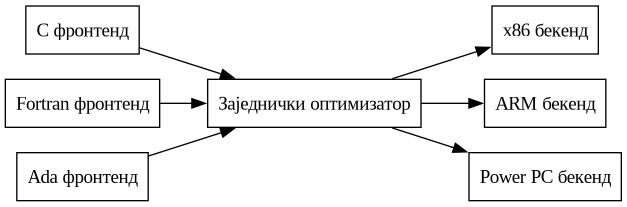
\includegraphics[width=5in, height=1.6in]{assets/images/modern_compiler_design.png}
\end{center}
\caption{Modularnost LLVM-a}
\label{lst:llvm_modular}
\end{listing}

Postoje brojne vrste optimizacije koje se mogu izvršiti nad izvornim kodom. Optimizacije se obično svode 
na tri osnovna koraka, pronalazak šablona koji se treba transformisati, validirati da li je bezbedno primeniti 
transformaciju i izvršavanje transformacije \cite{oss-architecture}. Optimizacije u \verb|LLVM| optmizatoru su modularne i izvršavaju 
se nad \verb|LLVM| medju reprezentacijom. Svaka \verb|LLVM| optmizacija je napisana kao \verb|C++| klasa koja 
nasledjuje \verb|Pass| (prolazak) klasu. Većina prolazaka je napisana u jedanom \verb|.cpp| fajlu.
Stoga otvara se mogućnost da se dodaju optimizacije specifične za jezik. Svaki prolazak se kompajlira u jedan 
ili više relokatabilnih objekata, (\verb|.o|) fajlova koji se potom grupišu u arhivne (\verb|.a|) fajlove. Objektni fajlovi 
su mašinski kod pre procesa linkovanja. Linkovanje je proces skupljanja i kombinovanja relokatabilnih objektnih fajlova
u jedan izvršni objektni fajl. Prilikom linkovanja nekog \verb|.o| fajla sa \verb|.a| fajlom linker će 
za svaki do tada nespojen simbol probati da nadje vezu u svim \verb|.o| fajlovima arhive.

\verb|LLVM| generator koda je odgovaran za prevodjenje \verb|LLVM| medju reprezentacije u mašinski kod ciljane 
arhitekture. Idealno za svaku arhitekturu postojao bi specifičan kod za prevodjenje, ali u isto vreme 
svi generatori rade vrlo sličan posao. Slično kao i kod optimizacije proces generisanja koda se deli u prolaske,
izbor seta instrukcija, način alokacije registara, planiranje (\verb|scheduling|), optimizacija rasporeda 
koda i generisanje asemblerskog koda. Pri kreiranju generatora za novu ciljnu arhitekturu svaki od ovih prolazaka
može ponovo da se iskoristi, modifikuje ili potpuno zameni.

\verb|LLVM| medju reprezentacija se veoma efikasno serijalizuje u i deserializuje iz \verb|LLVM| bitkoda. 
Ova efikasnost otvara mogućnost za optimizaciju u vreme linkovanja \ref{lst:link_time_opt}. To je još jedan set optimizacionih prolazaka 
koji dodatno poboljšava kranji mašinski kod. Linker prepoznaje da se u \verb|.o| fajlovima nalazi 
\verb|LLVM| bitkod umesto mašinskog koda, učitava ih u memoriju, linkuje ih, a potom izvršava \verb|LLVM|
optimizator nad mnogo većom celinom koda, omogućavajući daleko agresivnije optimizacije. 
Ova opcija se uključuje dodavanjem \verb|-O4| opcije komandne linije. 

\begin{listing}[H]
\begin{center}
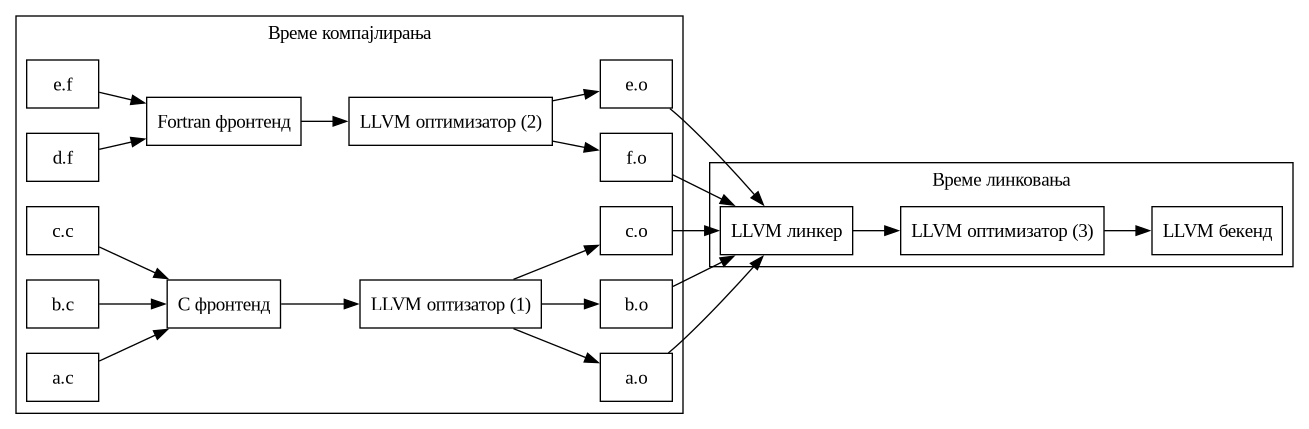
\includegraphics[width=6in, height=2.2in]{assets/images/link_time_optimization.png}
\end{center}
\caption{Optimizacija u vreme linkovanja}
\label{lst:link_time_opt}
\end{listing}

\verb|LLVM| medju reprezentacija podesća na asemblerski jezik. Strogo je tipiziran i poseduje jednostavne 
tipove poput celih brojeva, brojeva sa pokretnim zarezom, pokazivača i struktura. Jedna od glavnih razlika 
u odnosu na asembler jeste to što ne koristi ograničeni broj imenovanih registara već koristi beskonačan 
skup promenljivih koje se definišu sa \verb|%| prefiksom. Neki detalji mašine su apstrahovani od korisnika 
poput poziva funkcija (\verb|call|) i vraćanja vrednosti (\verb|ret|) \ref{lst:llvm_ir}.

\begin{listing}[H]
\begin{minted}{llvm}
define i32 @add2(i32 %a, i32 %b) {
entry:
  %tmp1 = icmp eq i32 %a, 0
  br i1 %tmp1, label %done, label %recurse

recurse:
  %tmp2 = sub i32 %a, 1
  %tmp3 = add i32 %b, 1
  %tmp4 = call i32 @add2(i32 %tmp2, i32 %tmp3)
  ret i32 %tmp4

done:
  ret i32 %b
}
\end{minted}
\caption{LLVM medju reprezentacija}
\label{lst:llvm_ir}
\end{listing}

\verb|Rust| jezik je \verb|frontend| nad \verb|LLVM|-om. Postoji puno olakšica u ovom pristupu.
\verb|Rust| tim ima cilj da izgeneriše pravilnu \verb|LLVM| medju reprezentaciju, na osnovu koje 
\verb|LLVM| izvršava optimizacione prolaske i generiše kod. Greške prilikom generisanja koda ne mora da 
održava \verb|Rust| tim, što značajno smanjuje količinu ljudi koja aktivno mora da bude uključena u razvoj. 
Svaka ciljna distribucija (arhitektura) koju \verb|LLVM| podržava automatski podržava i \verb|Rust|. Optimizacije se ne moraju 
posebno pisati i održavati jer \verb|LLVM| već poseduje značajan broj čestih optimizacija. \verb|Rust| 
omogućava kompajliranje na osnovu više \verb|LLVM| verzija, poslednja glavna verzija je uvek podržana,
i obično su podržane jedna ili dve ispod nje.
